\chapter{环形三相机视角插值方法}\label{chap:CVM_method}
视觉特效由于提供了独特的观赏体验,已经成为影视作品不可或缺的一部分。最著名的例子之一是《黑客帝国》中呈现的“子弹时间”效果。它创造了时间暂停的错觉,让观众似乎围绕演员转了一圈,并且视点平滑过渡。为了产生这种效果,160多个摄像头被同步和精确排列,这些相机通过一套高精度的激光对准系统在拍摄轨道上对齐,形成穿过空间的复杂拍摄曲线。然而,这种专门的采集系统造价昂贵,需要付出巨大的努力来建造。

视角插值算法能够使得“子弹时间”效果的建立更加灵活,\citet{seitz1996}在这方面的开创性工作指出,通过对两幅图像进行校正后再线性插值,能够实现保形的变换,如图~\ref{fig:view_morphing}。其中校正算法主要是为了降低像素匹配搜索的计算量,将匹配过程的搜索空间从二维降到一维。利用视角插值技术能大大降低使用相机的数量,只需要在轨迹上采样一定数量的相机,然后对每一对相邻的视图进行插值得到中间的帧。
现在考察相邻的两张图,整个视角插值的过程本质上还是需要从两幅图中推测3D几何信息。现有的方法中使用到的几何表达主要有轮廓信息、深度图和光流。这里对相邻图片要求要有较大的重叠区域,才能确保可靠的三维重建和插值。
\begin{figure}[!htbp]
    \centering
    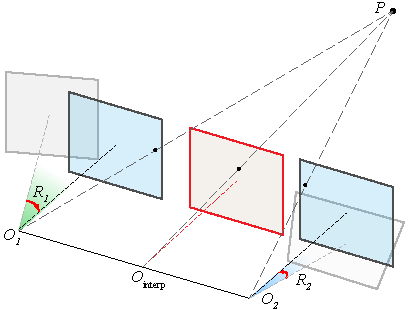
\includegraphics[width=0.60\textwidth]{view_morphing_fig1.pdf}
    \bicaption[视角插值过程示意图]{视角插值过程示意图。$O_1$,$O_2$代表两个相机的光心,$O_{\mathrm{interp}}$代表插值出的虚拟相机光心位置,两幅图像经过$R_1$,$R_2$旋转校正后能够线性插值出$P$在虚拟相机中的投影。}[Process of view morphing between two cameras]{Process of view morphing between two cameras.$O_1$,$O_2$ represent the principle point of input cameras, $O_{\mathrm{interp}}$ represents the virtual camera. After being rectified by $R_1$, $R_2$, the two rotation matrices,  The two reference cameras linearly interpolate the projection of $P$ in the virtual camera.}
    \label{fig:view_morphing}
\end{figure}
\citet{Ji_2017_CVPR}将视角插值的整个过程第一次端到端地放进了深度学习框架,利用训练数据中的冗余模式让网络自己学到了对图片的校正参数和匹配信息。但是到目前为止,这些方法还是一致假设相机路径为线性,并没有成功地展示360度的子弹时间效果。

本文中提出了一种新的同样基于深度学习,设计了能平滑且真实地进行视角变换的框架。这种方法使用最少三个参考图像沿圆弧形路径进行变换,如图~\ref{fig:real_setup}所示。
\begin{figure}[!htbp]
    \centering
    \includegraphics[width=\textwidth]{real_setup.pdf}
    \bicaption[采集系统]{采集系统。左边是需要大量相机的传统子弹时间采集系统示意图,右边是本文提出的方法的采集系统,在一个弧形路径上一组稀疏相机用来采集图像生成视角插值变换后的效果。}[Capturing system]{Capturing system. Left specialized acquisition system with numerous cameras is often needed forproducing the bullet-time effect; right shows the proposed method to morph transition images on acircular path from a sparse set of view samples for rendering such effect.}
    \label{fig:real_setup}
\end{figure}
本文采用了一种新的环形校正技术来将输入的三张图像校准到一个公共圆上,环形矫正后的图像具有最小投影失真的性质。然后将校正后的三张图喂给神经网络,用于新视图合成。本文提出的这个新的网络包含一个编解码结构,用于同时预测像素级运动场和可见性蒙版,还包含一个用于图像插值的混合网络。其中这个运动场和可见性蒙版共同构成了隐式几何表达。与传统的两张图像作为输入不同,本文通过使用第三张中间图像,可以可靠地处理遮挡和大面积的图像视角变化,其中最大的视角变化高达120度。

\section{环形校正}
传统的水平校正在立体匹配中很常见,能将对应匹配的搜索空间缩小到1D水平扫描线,这是因为校正后的图像可以认为是两个完全平行的摄像头直接拍摄得到的。但是这种方法对于围绕着一个物体进行拍摄的场景并不是适用,对于使用三张图片作为输入的情况也不是最优的。原因在于如果使用两两校正,那么三幅图像需要两两进行校正,那么对于一个相机来说会得到多个参数;另一个原因就是对于角度相差较大的两个相机,校正后边界可能出现较大的投影畸变。

本节提出新的环形校正方案,变换三张图像使得它们好像是由三个相机朝向一个公共圆的圆心拍摄的。由于三个不共线的点会确定出一个外接圆,那么总是可以从三个相机的光心坐标计算出这个圆。经过这样的变换后,像素的匹配同样被限制在一维的线上,不过这个线不再是水平。在接下来的过程中使用神经网络实现匹配过程,并将线扫描的约束加到了神经网络的训练中,以增加匹配精度。    

给定三张参考图像$\{\mathcal{I}_l, \mathcal{I}_m, \mathcal{I}_r\}$,以及相机的标定参数$\{K_i, R_i, t_i | i=l, m, r\}$,其中$K_i$是内参矩阵,$R_i$和$t_i$是外参中的旋转矩阵和相机光心坐标,下标$l, m, r$分别表达“左”,“中”和“右”,这是顺着圆弧从一端到另一端的顺序。首先使用相机的位置拟合外接圆的圆心,然后构造相应的单应性矩阵来对三张图像变换,图~\ref{fig:arc_rect}说明了这一过程。
\begin{figure}[!htbp]
    \centering
    \includegraphics[width=\textwidth]{arc_triplets_rectification-eps-converted-to.pdf}
    \bicaption[环形校正示意图]{环形校正示意图。三个相机沿弧形分布。经过环形校正后,参考图像被对齐到一个公共圆上,即它们的光轴都通过其外心,这三张图被称为弧三元组。}[Cyclic rectification]{Cyclic rectification. Three cameras are configured along a circular path for capturing the reference images. After cyclic rectification, the reference images are aligned on a common circle (i.e., their optical principal axes all pass through the circumcenter) and they are called the arc triplet.}
    \label{fig:arc_rect}
\end{figure}

\subsection{拟合公共圆的外心}
现在考虑三个相机光心构成的三角形,其外心理论上是三条边的垂直平分线交点。由于这三个相机是在同一世界坐标系下进行标定的,外参中的向量$\{t_i | i=l, m, r\}$物理意义就是相机光心。因此$\{t_i - t_j | i, j = l, r, m; i \neq j\}$就是三角形边的向量表达。首先通过公式(\ref{eq:eq_1})求解线性方程组得到外接圆平面的法向$\mathbf{n}$。
\begin{equation} \label{eq:eq_1}
    \adddotsbeforeeqnnum%
    \mathbf{n} \cdot (t_i - t_j) = 0
\end{equation}
接下来按照公式(\ref{eq:eq_2})计算垂直平分线归一后的单位方向向量。
\begin{equation}\label{eq:eq_2}
    \adddotsbeforeeqnnum%
    \mathbf{d}_{ij} = \frac{\mathbf{n} \times (t_i - t_j)}{\|t_i - t_j\|}
\end{equation}
最后圆心$O$的求解通过对三条垂直平分线$\{\mathbf{d}_{ij}|i,j=l, m, r; i \neq j\}$做三角化求交点得到,如公式(\ref{eq:eq_3})。
\begin{equation}\label{eq:eq_3}
    \adddotsbeforeeqnnum%
    O = \frac{1}{2}(t_i + t_j) + \alpha_{ij}\mathbf{d}_{ij}
\end{equation}
其中$\{\alpha_{ij}|i,j=l, m, r; i\neq j\}$是各边中点沿着垂线方向追踪出去的长度,在方程中为未知数,数量为三。观察方程可知九个方程求解三个未知数,显然是一个超定线性系统,本文使用奇异值分解(SVD)求解。

\subsection{单应性变换}
本小节推导用来变换三张图像$\{\mathcal{I}_l, \mathcal{I}_r, \mathcal{I}_m\}$的单应性矩阵$\{\mathit{H}_i|i=l, r, m\}$,使得校正后的图像朝向上节推出的外心$O$。具体来说对相机的变换包括两步旋转:首先将相机的$y$轴与平面的法向$\mathbf{n}$对齐,然后将相机的$z$轴指向外心$O$。给定初始的相机的轴向$\{\mathbf{x}_i, \mathbf{y}_i, \mathbf{z}_i\} | i=l, r, m$,这里三根轴向量与标定的旋转矩阵满足关系$R_i = [\mathbf{x}_i, \mathbf{y}_i, \mathbf{z}_i]$,可以如公式(\ref{eq:eq_4})计算出相机的三根轴经过对齐后的新坐标轴。
\begin{equation} \label{eq:eq_4}
    \adddotsbeforeeqnnum%
    \begin{cases}
        \mathbf{x}_i' = \mathbf{y}_i' \times \mathbf{z}_i'\\
        \mathbf{y}_i' = \mathrm{sgn}(\mathbf{n} \cdot \mathbf{y}_i) \cdot \mathbf{n}\\
        \mathbf{z}_i' = \mathrm{sgn}(\mathbf{z}_i \cdot ({O} - t_i)) \cdot \pi(O - t_i)
    \end{cases}
\end{equation}
这里$i = l, m, r$,同样作用于弧上的全部三个相机。$\mathrm{sgn}(\cdot)$是符号函数,$\pi(\cdot)$表示向量做归一化函数。通过坐标轴与外参旋转矩阵的关系得到新的旋转矩阵为$R_i' = [\mathbf{x}_i', \mathbf{y}_i', \mathbf{z}_i']$。变换图像的单应性矩阵$\{H_i | i=l, r, m\}$可以用公式(\ref{eq:eq_5})计算。
\begin{equation}\label{eq:eq_5}
    \adddotsbeforeeqnnum%
    H_i = K_iR_i'^{\top}R_iK_i^{-1}
\end{equation}
而图像的变换通过计算变换前后的像素坐标关系可得。假设变换前的齐次像素坐标$\tilde{\mathbf{u}}=[u_x, u_y, 1]^{\top}$,则变换后的其次像素坐标$\tilde{\mathbf{u}}'=H_i \tilde{\mathbf{u}}$。在实际实现的时候通常需要通过反向计算,即从变换后的像素坐标位置计算对应到原图像中的像素坐标,以拷贝颜色值。


\section{视角变换网络}
本节介绍新设计的用于视角变换的卷积网络,它以经过环形校正后的三幅图像作为输入,合成一个在弧上均匀分布的图像序列,能够光滑连续地插值出原本弧两端相机之间的视角,本文给新设计的这个网络以英文缩写CVMN代替,网络的结构如图~\ref{fig:cvmn_pipeline}所示。
\begin{figure}[!htbp]
    \centering
    \includegraphics[width=\textwidth]{pipeline-eps-converted-to.pdf}
    \bicaption[视角插值网络整体结构图]{视角插值网络整体结构图。该网络以环形校正后的弧上三元组为输入并合成连续平滑的新视角序列。}[Overall structure of CVMN]{The overall structure of Concyclic View Morphing Network (CVMN). It takes the arc triplet as input and synthesize sequence of concyclic views.}
    \label{fig:cvmn_pipeline}
\end{figure}
本节中将从输入的三元组$\{\mathcal{I}_i | i=l, m, r\}$经过环形校正得到的弧上三元组记作$\{\mathcal{C}_i | i=l, m, r\}$。由于$\{\mathcal{C}_i\}$ 总可以被视为是严格分布在一段圆弧上的,CVMN可以看作是专门针对环形设定下的插值器。它包括两个子模块:一个是用于估计像素级运动场$\{\mathcal{F}_i | i=1, \dots, N\}$,也就是隐式几何的编码器---解码器网络,这个模块同时还会预测可见性蒙版$\{\mathcal{M}_i | i=1, \dots, N$,其中$N$代表生成的连续图片序列的数量;另一个模块是一个融合图像的生成模块,专门用$\{\mathcal{C}_i, \mathcal{F}_i, \mathcal{M}_i | i = l, m, r\}$来合成最终的视角序列。

\subsection{编码器---解码器网络}
编码器---解码器结构被证明在建立像素点匹配方面是很有效\citep{Ilg_2017_CVPR, newell2016},因此本节也采用这种结构来预测用于插值中间视图的像素级运动矢量场$\mathcal{F}_i$,同时指出这种表达与几何之间的关系。首先使用一个编码器来提取输出的三元组$\mathcal{C}_i$的相关特征,然后使用双分支的解码器来分别估计运动矢量场和可见性蒙版,总体结构如图~\ref{fig:cvmn_encoder_decoder}所示。
\begin{figure}[!htbp]
    \centering
    \includegraphics[width=\textwidth]{net_overview-eps-converted-to.pdf}
    \bicaption[编码器---解码器模块结构图]{编码器---解码器模块结构图。将输入的三元组进行特征编码并交给后续两分支解码器预测。}[The encoder-decoder network]{The encoder-decoder network. The encoder transfer the arc triplet to feature tensor and two decoders predict the motion field and visibility masks.}
    \label{fig:cvmn_encoder_decoder}
\end{figure}

编码器采用Hourglass结构\citep{newell2016}以便于捕捉不同尺度的特征。这种对称的先自下而上(从高分辨率到低分辨率)而后自顶而下(从低分辨率到高分辨率)的结构支持后续的解码器输出像素级别的预测,而这样的局部到全局的过程会重复若干层,最后输出与输入相同的全分辨率特征张量。由于输入含有三张图,编码器会对每张图单独编码后再把三张图得到的特征连接在一起。另一种考量是先将三张图像接在一起再一起编码,这样方案会由于图片通道数量上升而使编码器的参数数量暴涨,对于有限的计算量来讲是不切实际的。对于输入的三元组来说,实际上它们共用了一个仅对单张图片编码的编码器。

运动场解码器接收从编码器输出的特征,并预测输出序列中每一张图的像素偏移。具体来讲考虑了两个运动场:一个是针对三元组中的左图$\mathcal{C}_l$,另一个是针对三元组中的右图$\mathcal{C}_r$。运动场实际上存储的是每一对匹配像素之间的偏移向量,并且为了减少由于非均匀离散采样造成的空洞,采用了反向映射的方式来计算,即计算从待求图像$\mathcal{C}_i$到目标图像$\mathcal{C}_l$或$\mathcal{C}_r$的位移矢量。以$\mathcal{C}_l$为例,现在考虑要插值出一张中间图像$\mathcal{C}_i$。假设已知一对特征匹配,像素$p_l=(x_l, y_l)$在图$\mathcal{C}_l$,像素$p_i=(x_i, y_i)$在图$\mathcal{C}_i$中,则偏移向量$\Delta_i^l(p)=(u_i^l(p), v_i^l(p))$符合公式(\ref{eq:shift})描述的关系。
\begin{equation}\label{eq:shift}
    \adddotsbeforeeqnnum%
    p_l = p_i + \Delta_i^l(p)
\end{equation}
类似地可以计算出对右图$\mathcal{C}_r$的偏移向量$\{\Delta_i^r(p)=(u_i^r(p), v_i^r(p)) | p = 1, \dots, M\}$,这里$M$表示一张图上的所有像素个数。将对$\mathcal{C}_l$和$\mathcal{C}_r$的偏移向量连接起来,得到本节定义的4D运动向量$[u_i^l(p), v_i^l(p), u_i^r(p), v_i^r(p)]$。这个定义是针对$\mathcal{C}_i$的一个像素而言,如果将所有的像素放在一起,消去像素$p$后得到四个标量场$\mathcal{F}_i=(U_i^l, V_i^l, U_i^r, V_i^r)$,这里$U_i^l=\{u_i^l(p)|i=1,\dots,N, p=1, \dots, M \}$,其余三个标量场依从类似的构造。

在网络的结构上,反卷积层和卷积层交替排列来从特征张量解码出运动场。这种中间层设计的原因是由于实验表明在反卷积层后面加入适当的卷积层可以减少输出图像中的马赛克样块状瑕疵。由于运动场共包含$\{U_i^l, V_i^l, U_i^r, V_i^r\}$四个标量场,需要用四个解码器实例各自独立预测一个标量场,这是为了避免不同物理含义的标量场之间产生不应该的关联。值得注意的是,在预测运动场时是需要引入对应中间图像$\mathcal{C}_m$的特征张量的,尽管去掉它整个流程也能跑通,但后续的实验表明$\mathcal{C}_m$对于提高运动场估计的精度有很大帮助。

可见性蒙版解码器主要用来预测像素级的可见性信息。在视角改变较大的情况下,不同视角的遮挡变化会在视角变换中造成可见性的问题,待插值位置的像素很可能在不同图像中各有一部分可见。如果直接对输入视图根据运动场信息做插值并融合,会造成“鬼影”瑕疵,因此需要引入可见性蒙版来解决这个问题。给定一个待输出图像$\mathcal{C}_i$,定义两个可见性蒙版$\mathcal{M}_i^l$和$\mathcal{M}_i^r$,用来表示表示逐像素的可见性水平,这个可见性水平是相对输入图像$\mathcal{C}_l$和$\mathcal{C}_r$的。数值越大,说明在参考图像中看到这个像素的概率越高。在数值的范围上,$\mathcal{M}_i^l$和$\mathcal{M}_i^r$并不严格遵循概率取值必须在0到1之间的约束,而是可以取任意大于零的数值。实验表明这种放松有助于网络在训练中收敛地更快更稳定。

可见性蒙版解码器同样由交替的反卷积和卷积层构成,并以编码器输出的特征为输入,这点与运动场解码器类似。不同之处在于在输出层之前使用额外的ReLU层来约束输出值必须大于零。对于针对左右两个输入图的可见性蒙版$\mathcal{M}^l$和$\mathcal{M}^r$,分别各需要一个解码器实例进行预测。

\subsection{融合网络}
融合网络模块最终合成输出视图序列$\{\mathcal{C}_i|i=1, \dots, N\}$,用的信息包括左右两幅输入图像$\mathcal{C}_l$和$\mathcal{C}_r$和两个解码器的输出$\{\mathcal{F}_i|i=1,\dots,N\}$和$\{\mathcal{M}_i|i=1,\dots,N\}$,这里$N$表示输出的插值图像序列的帧数。融合网络模块的架构如图~\ref{fig:cvmn_blending}所示,
\begin{figure}[!htbp]
    \centering
    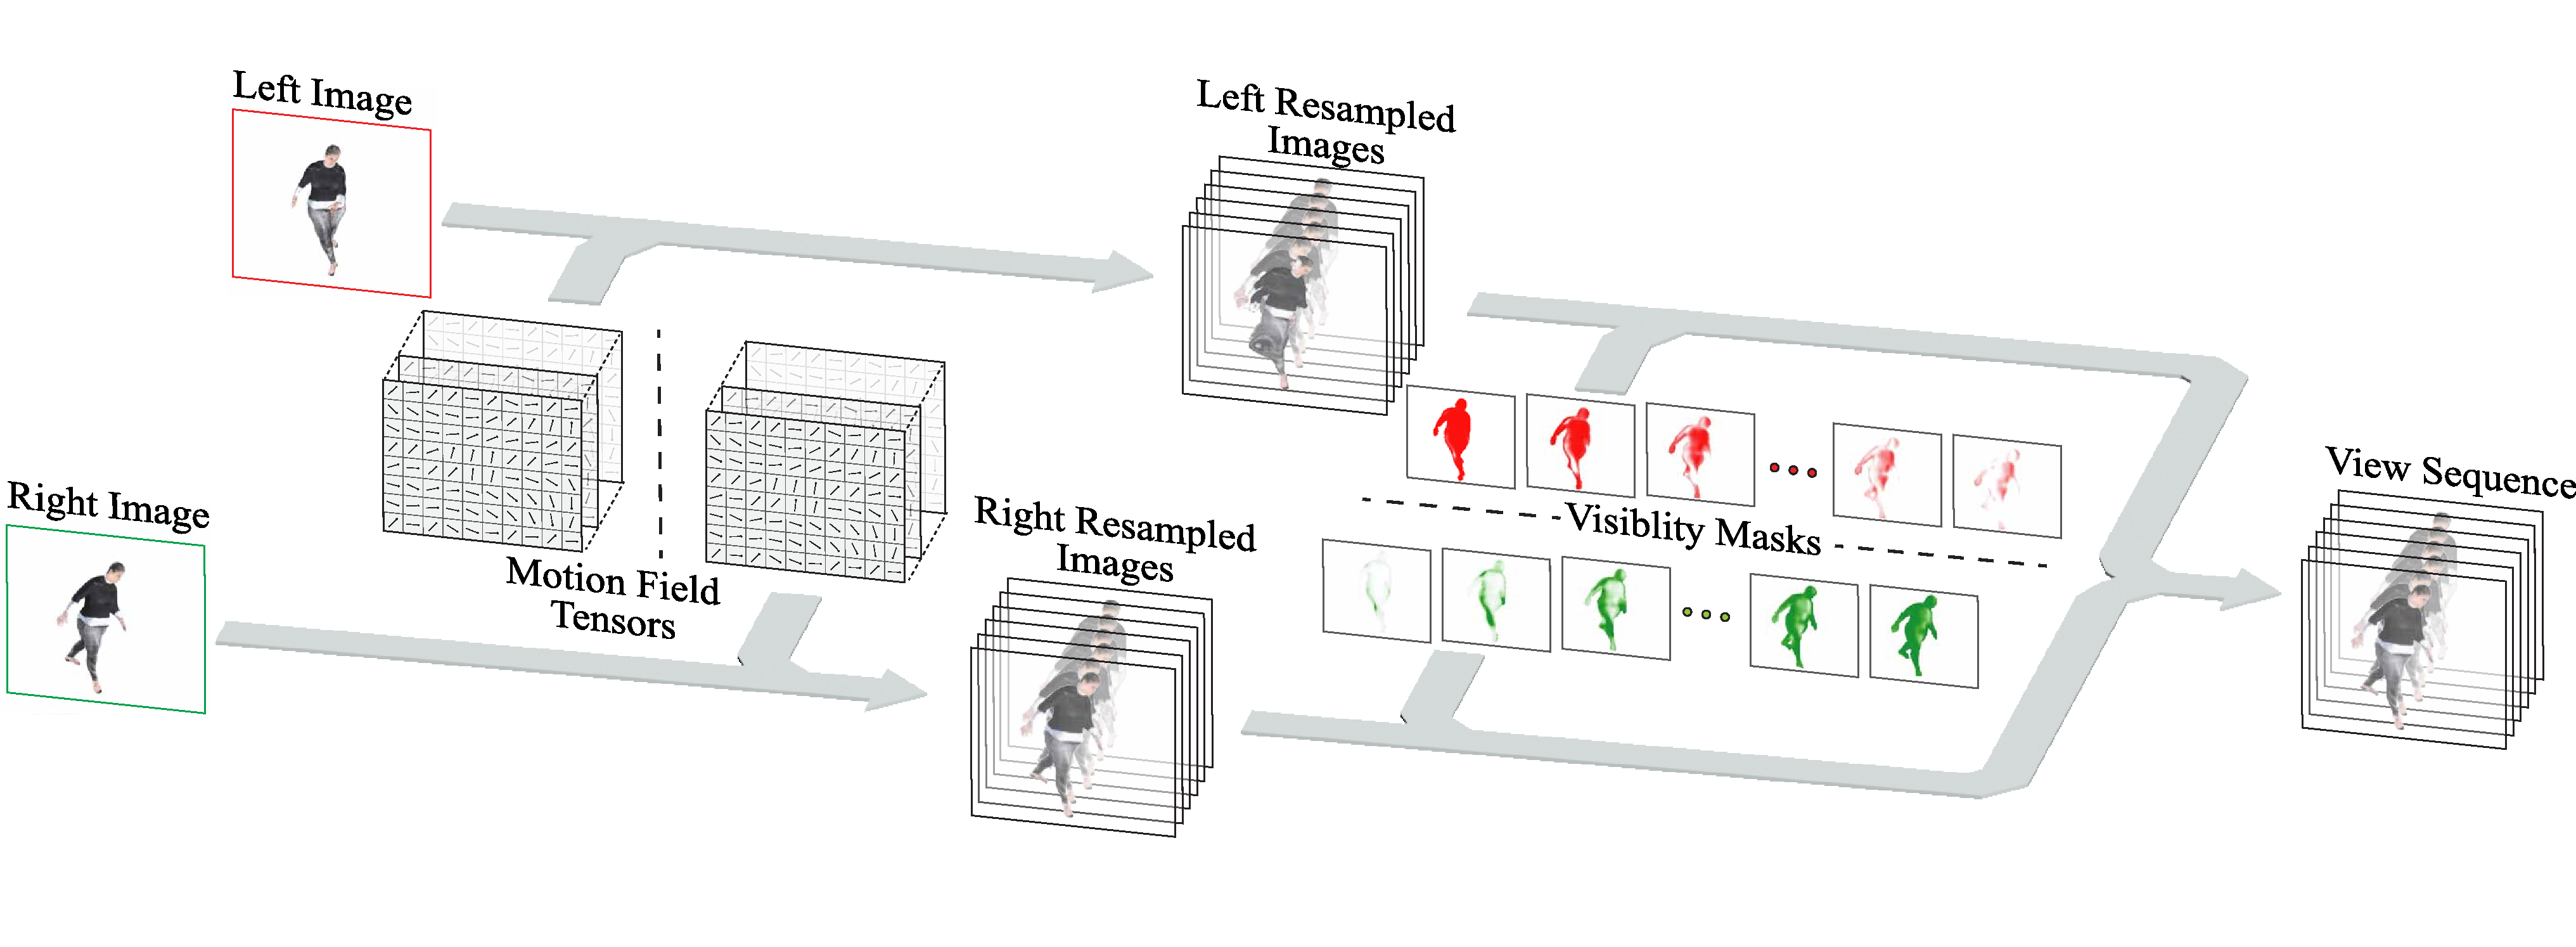
\includegraphics[width=\textwidth]{blending2.pdf}
    \bicaption[融合网络模块结构图]{融合网络模块结构图。利用预测的运动场信息和可见性蒙版信息合成插值帧序列。}[The blending network]{The blending network. Blending the morphed imaged using left reference image and right reference image, motion field and visibility masks.}
    \label{fig:cvmn_blending}
\end{figure}
首先由两个采样层对$\mathcal{C}_l$和$\mathcal{C}_r$进行重采样,重采样后的图像可以被公式$\mathcal{R}(\mathcal{C}_{\{l, r\}};U^{\{l, r\}}, V^{\{l, r\}})$表达,算子$\mathcal{R}(\cdot)$按照公式(\ref{eq:shift})对像素进行偏移量计算,对于每个新插值的视角,这会产生两幅重采样图像,一幅是从$\mathcal{C}_l$来的,一幅是从$\mathcal{C}_r$来的。接下来利用可见性蒙版$\mathcal{M}=(\mathcal{M}_l, \mathcal{M}_r)$作为权重,将重采样的图像加权融合。前面在描述可见性蒙版的时候提到解码器放松了蒙版的值域范围,因此这里需要做一步归一化操作,如公式(\ref{eq:eq_7})所示。
\begin{equation}\label{eq:eq_7}
    \adddotsbeforeeqnnum%
    \overline{\mathcal{M}}_i^{\{l, r\}} = \frac{\mathcal{M}_i^{\{l, r\}}}{\mathcal{M}_i^l + \mathcal{M}_i^r}
\end{equation}
这里的$i=1, \dots, N$。最终的合成图片序列可以通过公式(\ref{eq:eq_8})计算。
\begin{equation}\label{eq:eq_8}
    \adddotsbeforeeqnnum%
    \mathcal{C}_i = \mathcal{R}(\mathcal{C}_l; U_i^l, V_i^l) \otimes \overline{\mathcal{M}}_i^l + \mathcal{R}(\mathcal{C}_r; U_i^r, V_i^r) \otimes \overline{\mathcal{M}}_i^r
\end{equation}
运算$\otimes$代表逐像素的乘法。值得注意的是在整个融合模块里面所有的参数的运算都是固定的操作,没有任何可学习的参数,同时所有的计算都是连续可导的网络层,这意味着融合模块被链接进了整个神经网络且可以正常地进行反向传播操作。

\section{目标函数设计与隐式几何}
本节介绍网络训练的目标函数,为了引导CVMN的训练过程,设计目标函数的时候本方法考虑了三个方面的约束。第一个约束是合成的新视角的图片与真实值之间的相似度。由训练数据引入强约束,保证了能将数据集信息通过学习的方式融入网络参数,假设真实的监督视角图片记为$\{Y_i | i=1, \dots, N\}$,该约束直接比较图片之间的一范数,如公式(\ref{eq:eq_9})。
\begin{equation}\label{eq:eq_9}
    \adddotsbeforeeqnnum%
    \mathcal{L}_s = \sum_{i=1}^N \|Y_i - \mathcal{C}_i\|_1
\end{equation}
余下的两个约束均是从几何关系上推导出的,可以认为是不借助数据的自监督目标项,因此有必要先推导基于运动场与可见性的表达与三维几何的关系。以输入的左图$\mathcal{C}_l$为例,其内参矩阵$K_l$,外参旋转矩阵与光心坐标分别为$R_l$与$t_l$,待插值的图像$\mathcal{C}_i$,其内参矩阵$K_i$,外参旋转矩阵与光心坐标相应分别为$R_i$和$t_i$。现在考虑世界中的一点$P$,齐次像素坐标$\tilde{p_l}$和$\tilde{p_i}$分别表示在图中的位置,则满足公式(\ref{eq:epi})描述的关系。
\begin{equation} \label{eq:epi}
    \adddotsbeforeeqnnum%
    \begin{cases}
        P = R_l K_l^{-1}\tilde{p_l}d_l + t_l\\
        P = R_i K_i^{-1}\tilde{p_i}d_i + t_i
    \end{cases}
\end{equation}
其中$d_i$和$d_l$是点$P$在两个相机下各自的深度,而$p_i$实际上是由$p_l$和预测得到的运动场按照公式(\ref{eq:shift})描述。假设在上面式子里相机的内外参和像素坐标都是已知,那么将$P$、$d_i$和$d_l$视为未知数,整理两边可以得到六个线性方程,可以通过SVD分解快速求解出$d_i$和$d_l$。反过来如果知道$P$,则投影到两个相机的匹配像素点可以直接计算。

通过上面的论述明确了运动场计算出的偏移量作为隐式的几何表达,与直接给出3D点的位置在数学上是等价的。虽然计算3D点位置的计算复杂度相对更高,但这也是几乎所有隐式几何表达都有的一个特点。除此之外,当表达为偏移向量时,形式上可以将各个像素的偏移向量看作是以像素坐标为输入的二维函数,而这个函数显然是连续可导的,可以添加针对局部的光滑性约束。

现在介绍目标函数的第二个约束,该约束为从左右两个参考视图变换到当前图像时,来自左右的两幅变化图像之间的一致性。对于待插值出的每一辐图像$\mathcal{C}_i$,从左右参考图像$\mathcal{C}_l$和$\mathcal{C}_r$中各自能通过运动场变换出一张图像。尽管会出现遮挡变化,可是当注意力集中在可见区域时,在$\mathcal{C}_i$中某一像素,当其在左右图像中均为可见时候,这三个像素应该对应空间中同一个点,即从两边变换来的图像像素应该是基本一致的,由公式(\ref{eq:eq_11})表达。
\begin{equation} \label{eq:eq_11}
    \adddotsbeforeeqnnum%
    \mathcal{L}_u = \sum_{i=1}^N \|(\mathcal{R}_i^l - \mathcal{R}_i^r) \otimes \overline{\mathcal{M}}_i^l \otimes \overline{\mathcal{M}}_i^r \|_2^2
\end{equation}
这里使用两个可见性蒙版的乘法作为对可见性的置信近似,可以检验当某一像素对应的3D点在三张图中均为可见时,可见性权重相乘为1,而在其他情况下均小于1,且随可见性减小以二阶速度衰减到0。

第三个约束是运动场的估计应与参考图像之间满足对极几何约束,从公式(\ref{eq:epi})出发,消去$P$而仅关注$p_l$和$p_i$的关系如式(\ref{eq:eq_12})。
\begin{equation} \label{eq:eq_12}
    \adddotsbeforeeqnnum%
    R_l K_l^{-1}\tilde{p_l}d_l  =  R_i K_i^{-1}\tilde{p_i}d_i + (t_i - t_l)
\end{equation}
考虑同时在两边叉乘上$(t_i - t_l)$,为了表示叉乘,引入向量$t$对应的斜对称矩阵$\hat{t}$如公式(\ref{eq:eq_13})所示, 其中$t_1, t_2, t_3$表示三个分量,那么$t$叉乘上任意一个向量就等价于$\hat{t}$与该向量进行矩阵向量乘法。
\begin{equation} \label{eq:eq_13}
    \adddotsbeforeeqnnum%
    \hat{t} = \begin{bmatrix}
       0 & -t_3 & t_2  \\
       t_3 & 0  & -t_1 \\
       -t_2  & t_1 & 0
     \end{bmatrix}
\end{equation}
现在考虑公式(\ref{eq:eq_12})的两边同时叉乘上$(t_i - t_l)$,再将两边的$d_l$和$d_i$去掉,仅关注$p_l$与$p_i$之间的关系,则如公式(\ref{eq:eq_14})所示。
\begin{equation} \label{eq:eq_14}
    \adddotsbeforeeqnnum%
    (\hat{t_i} - \hat{t_l})R_l K_l^{-1}\tilde{p_l}  \sim  (\hat{t_i} - \hat{t_l})R_i K_i^{-1}\tilde{p_i}
\end{equation}
最后将偏移向量按照公式(\ref{eq:shift})代入,并观察公式(\ref{eq:eq_14})左边的向量按照数学定义应与$R_l K_l^{-1}\tilde{p_l}$垂直。以上分析都是以左图$\mathcal{C}_l$为例子,右图完全类似。由此此对极几何约束$\mathcal{L}_e$最终如公式(\ref{eq:eq_15})所示。
\begin{equation} \label{eq:eq_15}
\adddotsbeforeeqnnum%
    \begin{split}
        \mathcal{L}_e = \|\tilde{p_l}^\top K_l^{-\top} R_l^\top (\hat{t_i} - \hat{t_l})R_i K_i^{-1}(\tilde{p_l} + \tilde{\Delta}_i^l)\|^2 \\
       \qquad \qquad \qquad  + \|\tilde{p_r}^\top K_r^{-\top} R_r^\top (\hat{t_i} - \hat{t_r})R_i K_i^{-1}(\tilde{p_r} + \tilde{\Delta}_i^r)\|^2
    \end{split}
\end{equation}

将三个约束$\mathcal{L}_s$、$\mathcal{L}_u$和$\mathcal{L}_e$线性叠加起来就得到了如公式(\ref{eq:eq_16})所示的损失函数,其中$\lambda$和$\gamma$是平衡各个约束项的超参数。除开$\mathcal{L}_s$是直接衡量与真实数据的误差,其余两项分别是对运动场和可见性蒙版的约束,通过对设计的神经网络模块赋予物理和几何意义来强行使其在训练过程中满足相应的性质,以此达到将数据信息和先验知识结合的目的。
\begin{equation} \label{eq:eq_16}
\adddotsbeforeeqnnum%
        \mathcal{L} = \mathcal{L}_s + \lambda\mathcal{L}_u + \gamma\mathcal{L}_e 
\end{equation}

\section{本章小结}
本章介绍了结合深度学习和隐式几何表达的环形三相机视角变换插值的算法设计部分,包含新的三相机的环形校正算法和CVMN网络的整体结构。环形校正算法实际上将CVMN的输入统一变成了严格分布在圆弧上的三元组,缩小了网络需要处理的数据空间。CVMN网络又包括从图片中提取特征以及预测隐式几何表达的编解码器结构,以及无参数的且可导的融合生成模块。本章还介绍了针对CVMN的目标函数,能够同时被训练数据和隐式几何知识所约束,达到混合监督的目标。

